\documentclass[oneside]{amsbook}
\usepackage{amsthm, amsmath, amssymb}
\usepackage{geometry, setspace, graphicx, enumerate}
\usepackage{listings}
\onehalfspacing                 

\usepackage[usenames, dvipsnames]{color}
\definecolor{graphblue}{RGB}{52, 138, 189}
\definecolor{graphpurple}{RGB}{122, 104, 166}

\theoremstyle{plain}% default 
\newtheorem{thm}{Theorem}[chapter] 
\newtheorem{lem}[thm]{Lemma} 
\newtheorem{prop}[thm]{Proposition} 
\newtheorem{exer}[thm]{Exercise} 

\newtheorem*{cor}{Corollary} 

\theoremstyle{definition} 
\newtheorem{defn}[thm]{Definition}
\newtheorem{conj}[thm]{Conjecture}
\newtheorem{exmp}[thm]{Example}

\theoremstyle{remark} 
\newtheorem*{rem}{Remark} 
\newtheorem*{note}{Note} 
\newtheorem{case}{Case} 

\DeclareMathOperator*{\argmax}{arg\,max}
\DeclareMathOperator*{\argmin}{arg\,min}

\lstset{
language=Python,
numbers=left,
numberstyle=\scriptsize,
stepnumber=0,
numbersep=5pt,
showspaces=false,
breaklines=true,
basicstyle=\ttfamily\scriptsize,
frame=single,
commentstyle=\scriptsize,
prebreak=\raisebox{0ex}[0ex][0ex]{\ensuremath{\hookleftarrow}},
showstringspaces=false,
showtabs=false,
identifierstyle=\ttfamily,
stringstyle=\color{Gray},
commentstyle=\color{graphpurple},
keywordstyle=\color{graphblue},
commentstyle=\color{RoyalBlue},
keywordstyle=\color{RedViolet},
tabsize=2
}

\usepackage{hyperref}

\title{Elements of Statistical Learning}
\author{Andrew Tulloch}

\begin{document}
\maketitle

\tableofcontents

\setcounter{chapter}{1}
% Created by Andrew Tulloch

%!TEX TS-program = xelatex
%!TEX encoding = UTF-8 Unicode


\documentclass[12pt]{amsart}
\usepackage{amsthm, amsmath, amssymb}
\usepackage{geometry, setspace, graphicx, enumerate, fullpage}
\onehalfspacing                 
\usepackage{fontspec,xltxtra,xunicode}


% AMS Theorems
\theoremstyle{plain}% default 
\newtheorem{thm}{Theorem}[section] 
\newtheorem{lem}[thm]{Lemma} 
\newtheorem{prop}[thm]{Proposition} 
\newtheorem{exer}[thm]{Exercise} 

\newtheorem*{cor}{Corollary} 


\newcommand{\res}[2]{\text{Res}(#1,#2)}
\theoremstyle{definition} 
\newtheorem{defn}[thm]{Definition}
\newtheorem{conj}[thm]{Conjecture}
\newtheorem{exmp}[thm]{Example}

\theoremstyle{remark} 
\newtheorem*{rem}{Remark} 
\newtheorem*{note}{Note} 
\newtheorem{case}{Case} 

\newcommand{\expc}[1]{\mathbb{E}\left[#1\right]}
\newcommand{\var}{\text{Var}}
\newcommand{\cov}[1]{\text{Cov}\left(#1\right)}
\newcommand{\prob}[1]{\mathbb{P}(#1)}
\newcommand{\given}{ \, | \,}
\newcommand{\us}{0 \leq u \leq s}
\newcommand{\ts}[1]{\{ #1 \}}

\renewcommand{\phi}{\varphi}
\newcommand{\sigf}{\mathcal{F}}

\newcommand{\dzz}{\, dz}
\newcommand{\bigo}[1]{\mathcal{O}(#1)}

\newcommand{\al}{\alpha}
\newcommand{\Q}{\mathbb{Q}}
\newcommand{\R}{\mathbb{R}}
\newcommand{\C}{\mathbb{C}}
\newcommand{\Z}{\mathbb{Z}}
\newcommand{\E}{\mathbb{E}}
\newcommand{\N}{\mathbb{N}}

\newcommand{\I}{\mathbb{I}}

\renewcommand{\P}{\mathbb{P}}

\newcommand{\F}{\mathbb{F}}
\newcommand{\Ga}{\mathbb{G}}

\newcommand{\aut}[1]{\text{Aut}{(#1)}}

\newcommand{\gener}[1]{\langle #1 \rangle}
\newcommand{\charr}[1]{\text{char}(#1)}
\newcommand{\nth}{n\textsuperscript{th}}

\newcommand{\tworow}[2]{\genfrac{}{}{0pt}{}{#1}{#2}}
\newcommand{\xdeg}[2]{[#1 : #2]}
\newcommand{\gal}[2]{\text{Gal}(#1/#2)}
\newcommand{\minpoly}[2]{m_{#1, #2}(x)}

\newcommand{\mapping}[5]{\begin{align*}
	#1 : \quad     #2 &\rightarrow #3 \\
			#4  &\mapsto #5
\end{align*}	
}


\def\cip{\,{\buildrel p \over \rightarrow}\,} 
\def\cid{\,{\buildrel d \over \rightarrow}\,} 
\def\cas{\,{\buildrel a.s. \over \rightarrow}\,} 

\def\clp{\,{\buildrel L^p \over \rightarrow}\,} 

\def\eqd{\,{\buildrel d \over =}\,} 
\def\eqas{\,{\buildrel a.s. \over =}\,}

\newcommand{\sigg}{\mathcal{G}}		
\newcommand{\indic}[1]{\mathbf{1}_{\{ #1 \}} }
\newcommand{\itos}{\text{It\^o's\ }}
\DeclareMathOperator*{\argmax}{arg\,max}
\DeclareMathOperator*{\argmin}{arg\,min}

		
		
\title{Elements of Statistical Learning - Chapter Solutions}								% Document Title
\author{Andrew Tulloch}


\begin{document}
\maketitle
\section{Chapter 1}

No exercises.

\section{Chapter 2}
\begin{exer}
    Suppose that each of $K$-classes has an associated target $t_k$, which is a vector of all zeroes, except a one in the $k$-th position.  Show that classifying the largest element of $\hat y$ amounts to choosing the closest target, $\min_k \| t_k - \hat y \|$ if the elements of $\hat y$ sum to one. 
\end{exer}
\begin{proof}
    The assertion is equivalent to showing that \[
    \argmax_i \hat y_i = \argmin_k \| t_k - \hat y \| = \argmin_k \|\hat y - t_k \|^2
\] by monotonicity of $x \mapsto x^2$ and symmetry of the norm.  

WLOG, let $\| \cdot \|$ be the Euclidean norm $\| \cdot \|_2$.  Let $k = \argmax_i \hat y_i$, with $\hat y_k = \max y_i$.  Note that then $\hat y_k \geq \frac{1}{K}$, since $\sum \hat y_i = 1$.   

Then for any $k' \neq k$ (note that $y_{k'} \leq y_k$), we have \begin{align*}
    \| y - t_{k'} \|_2^2 - \| y - t_k \|_2^2 &= y_k^2 + \left(y_{k'} - 1 \right)^2 - \left( y_{k'}^2 + \left(y_k - 1 \right)^2 \right) \\
    &= 2 \left(y_k - y_{k'}\right) \\
    &\geq 0
\end{align*} since $y_{k'} \leq y_k$ by assumption.

Thus we must have \[
    \argmin_k \| t_k - \hat y \| = \argmax_i \hat y_i
\] as required.    
\end{proof}

\begin{exer}
    Show how to compute the Bayes decision boundary for the simulation example in Figure 2.5.
\end{exer}
\begin{proof}
    The Bayes classifier is \[
        \hat G(X) = \argmax_{g \in \mathcal G} P(g | X = x ).
    \] In our two-class example $\textsc{orange}$ and $\textsc{blue}$, the decision boundary is the set where \[
        P(g=\textsc{blue} | X = x) = P(g =\textsc{orange} | X = x) = \frac{1}{2}.
    \]  
    
    By the Bayes rule, this is equivalent to the set of points where \[
        P(X = x | g = \textsc{blue}) P(g = \textsc{blue}) = P(X = x | g = \textsc{orange}) P(g = \textsc{orange})
    \] And since we know $P(g)$ and $P(X=x|g)$, the decision boundary can be calculated.
\end{proof}
    
\begin{exer}
    Consider $N$ data points uniformly distributed in a $p$-dimensional unit ball centered at the origin.  Show the the median distance from the origin to the closest data point is given by \[
        d(p, N) = \left(1-\left(\frac{1}{2}\right)^{1/N}\right)^{1/p}
    \] 
\end{exer}
\begin{proof}
    Let $r$ be the median distance from the origin to the closest data point.  Then \[
        P(\text{All $N$ points are further than $r$ from the origin}) = \frac{1}{2}
    \] by definition of the median.

    Since the points $x_i$ are independently distributed, this implies that \[
        \frac{1}{2} = \prod_{i=1}^N P(\|x_i\| > r)
    \] and as the points $x_i$ are uniformly distributed in the unit ball, we have that \begin{align*}
        P(\| x_i \| > r) &= 1 - P(\| x_i \| \leq r) \\
                         &= 1 - \frac{Kr^p}{K} \\
                         &= 1 - r^p
    \end{align*}  Putting these together, we obtain that \[
        \frac{1}{2} = \left(1-r^p \right)^{N}
    \] and solving for $r$, we have \[
        r = \left(1-\left(\frac{1}{2}\right)^{1/N}\right)^{1/p}
    \]
\end{proof}

\begin{exer}
    Consider inputs drawn from a spherical multivariate-normal distribution $X \sim N(0,\mathbf{1}_p)$. The squared distance from any sample point to the origin has a $\chi^2_p$ distribution with mean $p$. Consider a prediction point $x_0$ drawn from this distribution, and let $a = \frac{x_0}{\| x_0\|}$ be an associated unit vector. Let $z_i = a^T x_i$ be the projection of each of the training points on this direction.
    Show that the $z_i$ are distributed $N(0,1)$ with expected squared distance from the origin 1, while the target point has expected squared distance $p$ from the origin.
    Hence for $p = 10$, a randomly drawn test point is about 3.1 standard deviations from the origin, while all the training points are on average one standard deviation along direction a. So most prediction points see themselves as lying on the edge of the training set.
\end{exer}

\begin{proof}
    Let $z_i = a^T x_i = \frac{x_0^T}{\| x_0 \|} x_i$.  Then $z_i$ is a linear combination of $N(0,1)$ random variables, and hence normal, with expectation zero and variance \[ 
        \text{Var}(z_i) = \| a^T \|^2 \text{Var}(x_i) = \text{Var}(x_i) = 1
    \] as the vector $a$ has unit length and $x_i \sim N(0, 1)$.
    
    For each target point $x_i$, the squared distance from the origin is a $\chi^2_p$ distribution with mean $p$, as required.  
\end{proof}

\begin{exer}
    \begin{enumerate}[(a)]
        \item Derive equation (2.27) in the notes.
        \item Derive equation (2.28) in the notes.
    \end{enumerate}
\end{exer}

\begin{proof}
    \begin{enumerate}[(i)]
        \item We have \begin{align*}
            EPE(x_0) &= E_{y_0 | x_0} E_{\mathcal{T}}(y_0 - \hat y_0)^2 \\
                     &= \text{Var}(y_0|x_0) + E_{\mathcal T}[\hat y_0 - E_{\mathcal T} \hat y_0]^2 + [E_{\mathcal T} - x_0^T \beta]^2 \\
                     &= \text{Var}(y_0 | x_0) + \text{Var}_\mathcal{T}(\hat y_0) + \text{Bias}^2(\hat y_0).
        \end{align*}  We now treat each term individually.  Since the estimator is unbiased, we have that the third term is zero.  Since $y_0 = x_0^T \beta + \epsilon$ with $\epsilon$ an $N(0,\sigma^2)$ random variable, we must have $\text{Var}(y_0|x_0) = \sigma^2$.  

        The middle term is more difficult.  First, note that we have \begin{align*}
            \text{Var}_{\mathcal T}(\hat y_0) &= \text{Var}_{\mathcal T}(x_0^T \hat \beta) \\
                    &= x_0^T \text{Var}_{\mathcal T}(\hat \beta) x_0 \\
                    &= E_{\mathcal T} x_0^T \sigma^2 (\mathbf{X}^T \mathbf{X})^{-1} x_0
            \end{align*} by conditioning (3.8) on $\mathcal T$.
        \item 
    \end{enumerate}
\end{proof}

\begin{exer}
    Consider a regression problem with inputs $x_i$ and outputs $y_i$, and a parameterized model $f_\theta(x)$ to be fit with least squares.  Show that if there are observations with \emph{tied} or \emph{identical} values of $x$, then the fit can be obtained from a reduced weighted least squares problem.
\end{exer}

\begin{proof}
    This is relatively simple.  WLOG, assume that $x_1 = x_2$, and all other observations are unique.  Then our RSS function in the general least-squares estimation is \[
        RSS(\theta) = \sum_{i=1}^N \left(y_i - f_\theta(x_i) \right)^2 = \sum_{i=2}^N w_i \left(y_i - f_\theta(x_i) \right)^2 
    \] where \[
        w_i = \begin{cases}
            2 & i = 2 \\
            1 & \text{otherwise}
        \end{cases}
    \]
    Thus we have converted our least squares estimation into a reduced weighted least squares estimation.  This minimal example can be easily generalised.
\end{proof}

\begin{exer}
    Suppose that we have a sample of $N$ pairs $x_i, y_i$, drawn IID from the distribution such that $x_i \sim h(x), y_i = f(x_i) + \epsilon_i, E(\epsilon_i) = 0, \text{Var}(\epsilon_i) = \sigma^2$.
    
    We construct an estimator for $f$ linear in the $y_i$, \[
        \hat f(x_0) = \sum_{i=1}^N \ell_i(x_0; \mathcal X) y_i
    \] where the weights $\ell_i(x_0; X)$ do not depend on the $y_i$, but do depend on the training sequence $x_i$ denoted by $\mathcal X$.  
    \begin{enumerate}[(a)]
        \item Show that the linear regression and $k$-nearest-neighbour regression are members of this class of estimators.  Describe explicitly the weights $\ell_i(x_0; \mathcal X)$ in each of these cases.
    \end{enumerate}
\end{exer}

\begin{proof}
    \begin{enumerate}[(a)]
        \item Recall that the estimator for $f$ in the linear regression case is given by \[
            \hat f(x_0) = x_0^T \beta 
        \] where $\beta = (X^T X)^{-1} X^T y$.  Then we can simply write \[
            \hat f(x_0) = \sum_{i=1}^N \left( x_0^T (X^T X)^{-1} X^T \right)_i y_i.
        \]  Hence \[
            \ell_i(x_0; \mathcal X) = \left( x_0^T (X^T X)^{-1} X^T \right)_i.
        \]
        
        In the $k$-nearest-neighbour representation, we have \[
            \hat f(x_0) = \sum_{i=1}^N \frac{y_i}{k} \mathbf{1}_{x_i \in N_k(x_0)}
        \] where $N_k(x_0)$ represents the set of $k$-nearest-neighbours of $x_0$.  Clearly, \[
            \ell_i(x_0; \mathcal X) = \frac{1}{k} \mathbf{1}_{x_i \in N_k(x_0)}
        \]
    \end{enumerate}
\end{proof}
\end{document}

\documentclass[12pt]{amsart}
\usepackage{amsthm, amsmath, amssymb}
\usepackage{geometry, setspace, graphicx, enumerate, fullpage}
\usepackage{listings}
\onehalfspacing                 

\usepackage[usenames, dvipsnames]{color}
\definecolor{graphblue}{RGB}{52, 138, 189}
\definecolor{graphpurple}{RGB}{122, 104, 166}

\theoremstyle{plain}% default 
\newtheorem{thm}{Theorem}[section] 
\newtheorem{lem}[thm]{Lemma} 
\newtheorem{prop}[thm]{Proposition} 
\newtheorem{exer}[thm]{Exercise} 

\newtheorem*{cor}{Corollary} 

\theoremstyle{definition} 
\newtheorem{defn}[thm]{Definition}
\newtheorem{conj}[thm]{Conjecture}
\newtheorem{exmp}[thm]{Example}

\theoremstyle{remark} 
\newtheorem*{rem}{Remark} 
\newtheorem*{note}{Note} 
\newtheorem{case}{Case} 

\DeclareMathOperator*{\argmax}{arg\,max}
\DeclareMathOperator*{\argmin}{arg\,min}

\lstset{
language=Python,
numbers=left,
numberstyle=\scriptsize,
stepnumber=0,
numbersep=5pt,
showspaces=false,
breaklines=true,
basicstyle=\ttfamily\scriptsize,
frame=single,
commentstyle=\scriptsize,
prebreak=\raisebox{0ex}[0ex][0ex]{\ensuremath{\hookleftarrow}},
showstringspaces=false,
showtabs=false,
identifierstyle=\ttfamily,
stringstyle=\color{Gray},
commentstyle=\color{graphpurple},
keywordstyle=\color{graphblue},
commentstyle=\color{RoyalBlue},
keywordstyle=\color{RedViolet},
tabsize=2
}

\title{Elements of Statistical Learning - Chapter 3 Solutions}								% Document Title
\author{Andrew Tulloch}

\begin{document}
\maketitle
\setcounter{section}{2}

\section{Chapter 3}

\begin{exer}
  Show that the $F$ statistic for dropping a single coefficient from a model is equal to the square of the corresponding $z$-score.
\end{exer}

\begin{proof}
  Recall that the $F$ statistic is defined by the following expression \[
    \frac{(RSS_0 - RSS_1) / (p_1 - p_0)}{RSS_1 / (N - p_1 - 1)}.
  \] where $RSS_0, RSS_1$ and $p_0 + 1, p_1 + 1$ refer to the residual sum of squares and the number of free parameters in the smaller and bigger models, respectively.  Recall also that the $F$ statistic has a $F_{p_1 - p_0, N-p_1 - 1}$ distribution under the null hypothesis that the smaller model is correct.

  Next, recall that the $z$-score of a coefficient is \[
    z_j = \frac{\hat \beta_j}{\hat \sigma \sqrt{v_j}}
  \] and under the null hypothesis that $\beta_j$ is zero, $z_j$ is distributed according to a $t$-distribution with $N-p-1$ degrees of freedom. 

  Hence, by dropping a single coefficient from a model, our $F$ statistic has a $F_{1, N-p - 1}$ where $p + 1$ are the number of parameters in the original model.  Similarly, the corresponding $z$-score is distributed according to a $t_{N-p-1}$ distribution, and thus the square of the $z$-score is distributed according to an $F_{1, N-p-1}$ distribution, as required.

  Thus both the $z$-score and the $F$ statistic test identical hypotheses under identical distributions.  Thus they must have the same value in this case.    

\end{proof}
\begin{exer}
    Given data on two variables $X$ and $Y$, consider fitting a cubic polynomial regression model $f(X) = \sum_{j=0}^{3} \beta_j X^j$.  In addition to plotting the fitted curve, you would like a 95\% confidence band about the curve.  Consider the following two approaches:
\begin{enumerate}
    \item At each point $x_0$, form a 95\% confidence interval for the linear function $a^T \beta = \sum_{j=0}^{3}\beta_j x_0^j$.  
    \item Form a 95\% confidence set for $\beta$ as in (3.15), which in tun generates confidence intervals for $f(x_0)$.  
\end{enumerate}
   How do these approaches differ?  Which band is likely to be wider?  Conduct a small simulation experiment to compare the two methods.
\end{exer}

\begin{proof}
    The key distinction is that in the first case, we form the set of points such that we are 95\% confident that $\hat f(x_0)$ is within this set, whereas in the second method, we are 95\% confident that an arbitrary point is within our confidence interval.  This is the distinction between a \emph{pointwise} approach and a \emph{global} confidence estimate. 
    
    In the pointwise approach, we seek to estimate the variance of an individual prediction - that is, to calculate $\text{Var}(\hat f(x_0) | x_0)$.  Here, we have \begin{align*}
        \sigma_0^2 = \text{Var}(\hat f(x_0) | x_0) &= \text{Var}(x_0^T \hat \beta | x_0) \\
                                    &= x_0^T \text{Var}(\hat \beta) x_0 \\
                                    &= \hat \sigma^2 x_0^T (X^T X)^{-1} x_0.
    \end{align*} where $\hat \sigma^2$ is the estimated variance of the innovations $\epsilon_i$.
    
    
    \begin{figure}
	\centering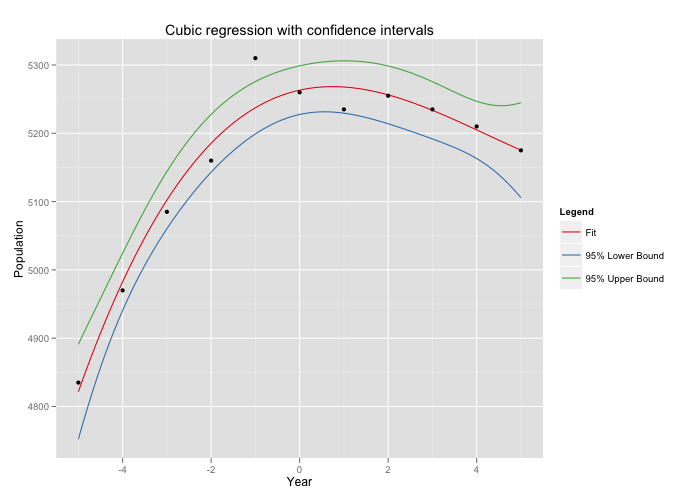
\includegraphics[width=\textwidth]{./RCode/CubicRegression.png}
    \end{figure}

    We can implement this algorithm in R as follows:

\begin{lstlisting}
library("ggplot2")
library("reshape2")

# Raw data
simulation.xs <- c(1959, 1960, 1961, 1962, 1963, 1964, 1965, 1966, 1967, 1968, 1969)
simulation.ys <- c(4835, 4970, 5085, 5160, 5310, 5260, 5235, 5255, 5235, 5210, 5175)
simulation.df <- data.frame(pop = simulation.ys, year = simulation.xs)

# Rescale years
simulation.df$year <- simulation.df$year - 1964

# Generate regression, construct confidence intervals
fit <- lm(pop ~ year + I(year^2) + I(year^3), data=simulation.df)
xs <- seq(-5, 5, 0.1)
fit.confidence <- predict(fit, data.frame(year=xs), interval="confidence", level=0.95)


# Create data frame containing variables of interest
df <- as.data.frame(fit.confidence)
df$year <- xs
df <- melt(df, id.vars="year")

p <- ggplot()
p <- p + geom_line(aes(x=year, y=value, colour=variable),
                   df)
P <- p + geom_point(aes(x=year, y=pop), 
                    simulation.df)
p <- p + scale_x_continuous('Year') 
p <- p + scale_y_continuous('Population')
p <- p + opts(title="Cubic regression with confidence intervals")
p <- p + scale_color_brewer(name="Legend",
        labels=c("Fit", 
                 "95% Lower Bound", 
                 "95% Upper Bound"), 
        palette="Set1")
\end{lstlisting}
\end{proof}

\begin{exer}
    Prove the Gauss-Markov theorem: the least squares estimate of a parameter $a^T\beta$ has a variance no bigger than that of any other linear unbiased estimate of $a^T\beta$.

    Secondly, show that if $\hat V$ is the variance-covariance matrix of the least squares estimate of $\beta$ and $\tilde V$ is the variance covariance matrix of any other linear unbiased estimate, then $\hat V \leq \tilde V$, where $B \leq A$ if $A - B$ is positive semidefinite.
\end{exer}

\begin{proof}
    Let $\hat \theta = a^T \hat \beta = a^T(X^TX)^{-1}X^T y$ be the least squares estimate of $a^T \beta$.  Let $\tilde \theta = c^T y$ be any other unbiased linear estimator of $a^T \beta$.  Now, let $d^T = c^T - a^T(X^{-1}X)^{-1}X^T$.  Then as $c^T y$ is unbiased, we must have \begin{align*}
        E(c^T y) &= E\left( a^T(X^{T}X)^{-1}X^T + d^T\right) y \\
                &= a^T\beta + d^T X\beta \\
                &= a^T\beta
    \end{align*} as $c^T y$ is unbiased, which implies that $d^T X = 0$.

    Now we calculate the variance of our estimator.  We have \begin{align*}
        \text{Var}(c^T y) &= c^T \text{Var}(y) c \\
                    &= \sigma^2 c^T c \\
                    &= \sigma^2 \left( a^T(X^{T}X)^{-1}X^T + d^T \right) \left( a^T (X^T X)^{-1} X^T + d^T \right)^T \\
                    &= \sigma^2 \left( a^T (X^T X)^{-1}X^T + d^T\right) \left(X (X^{T}X)^{-1}a + d\right) \\
                    &= \sigma^2 \left( a^T (X^TX)^{-1}X^T X(X^T X)^{-1} a + a^T (X^T X)^{-1} \underbrace{X^T d}_{=0} + \underbrace{d^T X}_{=0}(X^T X)^{-1} a + d^T d \right) \\
                    &= \sigma^2 \left(\underbrace{a^T (X^T X)^{-1} a}_{\text{Var}(\hat \theta)} + \underbrace{d^t d}_{\geq 0} \right)
    \end{align*}

    Thus $\text{Var}(\hat \theta) \leq \text{Var}(\tilde \theta)$ for all other unbiased linear estimators $\tilde \theta$.

    The proof of the matrix version is almost identical, except we replace our vector $d$ with a matrix $D$.  It is then possible to show that $\tilde V = \hat V + D^T D$, and as $D^T D$ is a positive semidefinite matrix for any $D$, we have $\hat V \leq \tilde V$. 
\end{proof}

\begin{exer}
    Show how the vector of least square coefficients can be obtained from a single pass of the Gram-Schmidt procedure.  Represent your solution in terms of the QR decomposition of $X$.  
\end{exer}

\begin{proof}
    Recall that by a single pass of the Gram-Schmidt procedure, we can write our matrix $X$ as \[
        X = Z \Gamma,
        \] where $Z$ contains the orthogonal columns $z_j$, and $\Gamma$ is an upper-diagonal matrix with ones on the diagonal, and $\gamma_{ij} = \frac{\langle z_i, x_j \rangle}{\| z_i \|^2}$. This is a reflection of the fact that by definition, \[
            x_j = z_j + \sum_{k=0}^{j-1} \gamma_{kj} z_k.
            \]

            Now, by the $QR$ decomposition, we can write $X = QR$, where $Q$ is an orthogonal matrix and $R$ is an upper triangular matrix.  We have $Q = Z D^{-1}$ and $R = D\Gamma$, where $D$ is a diagonal matrix  with $D_{jj} = \| z_j \|$.  

    Now, by definition of $\hat \beta$, we have \[
        (X^T X) \hat \beta = X^T y.
        \]  Now, using the $QR$ decomposition, we have \begin{align*}
            (R^T Q^T) (QR) \hat \beta &= R^T Q^T y \\
            R \hat \beta &= Q^T y
        \end{align*}
    As $R$ is upper triangular, we can write \begin{align*}
        R_{pp} \hat \beta_p &= \langle q_p, y \rangle \\
        \| z_p \| \hat \beta_p &= \| z_p \|^{-1} \langle z_p, y \rangle \\
        \hat \beta_p &= \frac{\langle z_p, y \rangle}{\| z_p \|^2}
    \end{align*} in accordance with our previous results.  Now, by back substitution, we can obtain the sequence of regression coefficients $\hat \beta_j$.  As an example, to calculate $\hat \beta_{p-1}$, we have \begin{align*}
        R_{p-1, p-1} \hat \beta_{p-1} + R_{p-1,p} \hat \beta_p &= \langle q_{p-1}, y \rangle \\
        \| z_{p-1} \| \hat \beta_{p-1} + \| z_{p-1} \| \gamma_{p-1,p} \hat \beta_p &= \| z_{p-1} \|^{-1} \langle z_{p-1}, y \rangle 
    \end{align*} and then solving for $\hat \beta_{p-1}$. This process can be repeated for all $\beta_j$, thus obtaining the regression coefficients in one pass of the Gram-Schmidt procedure.
\end{proof}

\begin{exer}
    Consider the ridge regression problem (3.41).  Show that this problem is equivalent to the problem \[
        \hat \beta^c = \argmin_{\beta^c} \left( \sum_{i=1}^{N} \left( y_i - \beta^c_0 - \sum_{j=1}^{p}(x_{ij} - \hat x_j) \beta^c_j \right)^2 + \lambda \sum_{j=1}^{p}{\beta_j^c}^2 \right)^2.
        \]
\end{exer}

\begin{proof}
    Consider rewriting our objective function above as  \[
        L(\beta^c) = \sum_{i=1}^{N}\left(y_i - \left(\beta_0^c - \sum_{j=1}^{p} \bar x_j \beta_j^c \right) - \sum_{j=1}^p x_{ij} \beta_j^c \right)^2 + \lambda \sum_{j=1}^p {\beta_j^2}^2
        \]
    Note that making the substitutions \begin{align*}
        \beta_0 &\mapsto \beta_0^c - \sum_{j=1}^p \hat x_j \beta_j \\
        \beta_j &\mapsto \beta^c_j, j = 1, 2, \dots, p
    \end{align*} that $\hat \beta$ is a minimiser of the original ridge regression equation if $\hat \beta^c$ is a minimiser of our modified ridge regression.  

    The modified solution merely has a shifted intercept term, and all other coefficients remain the same.  
\end{proof}

\begin{exer}[Exercise 3.12]
    For our augmented matrix $X_1$, equal to appending $\sqrt{\lambda I}$ to the original observation matrix $X$, we have that the $RSS$ expression for OLS regression becomes \begin{align*}
        RSS &= \sum_{i=1}^{N+p} \left(y_i - \sum_{j=1}^p x_{ij} \beta_j \right)^2 \\
            &= \sum_{i=1}^{N} \left( y_i - \sum_{j=1}^p x_{ij} \beta_j \right)^2 + \sum_{i = N + 1}^{N+p} \left(\sum_{j=1}^p x_{ij} \beta_j \right)^2 \\
            &= \sum_{i=1}^{N} \left( y_i - \sum_{j=1}^p x_{ij} \beta_j \right)^2 + \sum_{j=1}^p \lambda \beta_j^2 
    \end{align*} which is the objective function for the ridge regression estimate.
\end{exer}

\end{document}


\end{document}
